%%----------------------------------------------------------------------------
%% Onderzoekstechnieken: Tijdreeksen
%%----------------------------------------------------------------------------

\documentclass[aspectratio=169]{beamer}

%==============================================================================
% Aanloop
%==============================================================================

%---------- Vormgeving --------------------------------------------------------

\usetheme{hogent}

\usecolortheme{hgwhite} % witte achtergrond, zwarte tekst

\usepackage{graphicx,multicol}
\usepackage{comment,enumerate,hyperref}
\usepackage{amsmath,amsfonts,amssymb}
\usepackage[english]{babel}
\usepackage{multirow}
\usepackage{eurosym}
\usepackage{listings}
\usepackage{textcomp}
\usepackage{framed}
\usepackage{wrapfig}
\usepackage{tabu} %needed for \tabulinesep
\usepackage{wrapfig}
\usepackage{pgf-pie}
\usepackage{pgfplots}
\usepackage{booktabs}
\usepackage{pgfplotstable}
\usepackage{changepage}
\usepackage{ulem} % for \sout{text} (strikethrough)
\usepackage{fancyvrb} % for \begin{Verbatim} (LaTeX controls within verbatim)

%---------- Configuratie ------------------------------------------------------

\pgfplotsset{compat=1.16}
\usetikzlibrary{arrows,shapes,backgrounds,positioning,shadows}
\usetikzlibrary{pgfplots.statistics}

%---------- Commando-definities -----------------------------------------------

\newcommand{\tabitem}{~~\llap{\textbullet}~~}
\newcommand{\alertbox}[2][hgblue]{%
  \setbeamercolor{alertbox}{bg=#1,fg=white}
  \begin{beamercolorbox}[sep=2pt,center]{alertbox}
    \textbf{#2}
  \end{beamercolorbox}
}
\pgfmathdeclarefunction{gauss}{2}{%
  \pgfmathparse{1/(#2*sqrt(2*pi))*exp(-((x-#1)^2)/(2*#2^2))}%
}

%---------- Info over de presentatie ------------------------------------------

\title{Chapter 7. Time Series}
\subtitle{Research Techniques}
\author{Jens Buysse \and Pieter-Jan Maenhaut \and Bert {Van Vreckem}}
\date{AY 2020-2021}

%==============================================================================
% Inhoud presentatie
%==============================================================================

\begin{document}

\begin{frame}
  \maketitle
\end{frame}

\begin{frame}
  \frametitle{What's on the menu?}
  
  \tableofcontents
\end{frame}

\begin{frame}
  \frametitle{Learning Goals}
  
  \begin{itemize}
    \item Concepts, time series models
    \item Moving average
    \item Exponential smoothing
  \end{itemize}
\end{frame}


\section{Time series and predictions}

\begin{frame}
  \frametitle{Time series and predictions}
  
  \alertbox{A time series is a sequence of observations of an arbitrary variable in time order.}
  
  A time series is a stochastic process. Examples:
  
  \begin{itemize}
    \item Monthly demand for milk
    \item Annual intake of students at HOGENT
    \item Price of a share or bond on the stock exchange (hourly, daily, \dots)
    \item Number of HTTP requests per second for a website
    \item Evolution of disk usage on a backup server
  \end{itemize}
\end{frame}

\begin{frame}
  \frametitle{Time series and predictions}
  
  Time series are an import aspect of research, because they often form the \textbf{basis} for decision models and predictions.
  
  \begin{itemize}
    \item general development of future plans (investments, capacity \dots)
    \item budget planning to avoid shortcomings (operating budget, marketing budget \dots)
    \item support for financial objectives
    \item avoid uncertainty
  \end{itemize}
\end{frame}

\begin{frame}[plain]
  \frametitle{Time series and predictions}
  
  Time series are a \textbf{statistical} problem: observations vary with time
  
  \begin{figure}
    \centering
    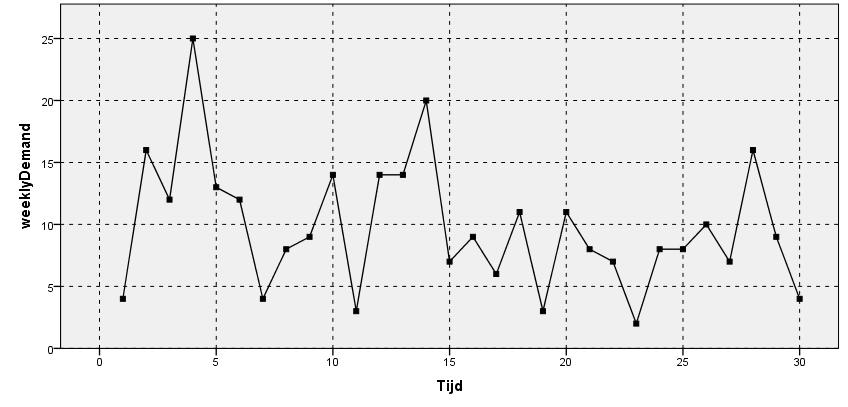
\includegraphics[height=.5\textheight]{tijdreeks11}
    \caption{Time series for the weekly demand for a particular product}
  \end{figure}
\end{frame}

\section{Time series models}

\subsection{Mathematical model}

\begin{frame}
  \frametitle{Mathematical model time series}
  
  The simplest model:
  
  \begin{itemize}
    \item Constant $b$
    \item Variations around $b$ determined by a random variable $\varepsilon_{t}$
  \end{itemize}
  
  \begin{equation}
  X_{t} = b + \varepsilon_{t}
  \label{eq:time-series-constant}
  \end{equation}
  
  \begin{itemize}
    \item $X_{t}$: stochastic variable for time series, at time $t$
    \item $x_{t}$: \textbf{observation} at time $t$ (known!)
    \item $\varepsilon_{t}$ is called the \textbf{noise}. We assume that $\varepsilon_{t} \sim Nor(\mu = 0; \sigma)$
  \end{itemize}
\end{frame}

\begin{frame}
  \frametitle{Mathematical model time series}
  
  We could also assume that there is a linear relationship:
  
  \begin{equation}
  X_{t} = b_{0} + b_{1} \times t + \varepsilon_{t}
  \label{eq:time-series-linear}
  \end{equation}
  
  Equation~\ref{eq:time-series-constant} and \ref{eq:time-series-linear} are special cases of the \textbf{polynomial} case:
  
  \begin{equation}
  X_{t} = b_{0} + b_{1} t + b_{2} t^{2} + \dots + b_{n} t^{n} + \varepsilon_{t}
  \label{eq:time-series-polynomial}
  \end{equation}
\end{frame}

\subsection{General}

\begin{frame}
  \frametitle{General expression time series}
  
  \begin{equation}
  X_{t} = f(b_{0}, b_{1}, b_{2}, \dots , b_{n}, t) + \varepsilon_{t}
  \label{eq:time-series-general}
  \end{equation}
  
  We make these assumptions:
  
  \begin{itemize}
    \item We consider two components of variability:
    \begin{itemize}
      \item the mean of the predictions changes with time
      \item the variations to this mean vary randomly
    \end{itemize}
    \item The residuals of the model ($X_t - x_t$) have a constant variance in time (\textbf{homoscedatic})
  \end{itemize}
\end{frame}

\subsection{Estimating the parameters}

\begin{frame}
  \frametitle{Estimating the parameters}
  
  Make \textbf{predictions} based on the time series model:
  
  \begin{enumerate}
    \item select the most suitable model
    \item estimation for parameters $b_i (i: 1, \dots, n)$ based on observations
  \end{enumerate}
  
  The estimations $\widehat{b_i}$ are selected so that they approximate the observed values as close as possible.
\end{frame}

\begin{frame}
  \frametitle{Example}
  
  \begin{table}[t]
    \centering
    \begin{tabular}{|l|l|l|l|l|l|l|l|l|l|}
      \hline
      4 & 16 & 12 & 25 & 13 & 12 & 4 & 8  & 9 & 14 \\ \hline
      3 & 14 & 14 & 20 & 7  & 9  & 6 & 11 & 3 & 11 \\ \hline
      8 & 7  & 2  & 8  & 8  & 10 & 7 & 16 & 9 & 4  \\ \hline
    \end{tabular}
    \label{tab:data}
    \caption{Time series for the weekly demand for a product}
  \end{table}
  
  \begin{figure}
    \centering
    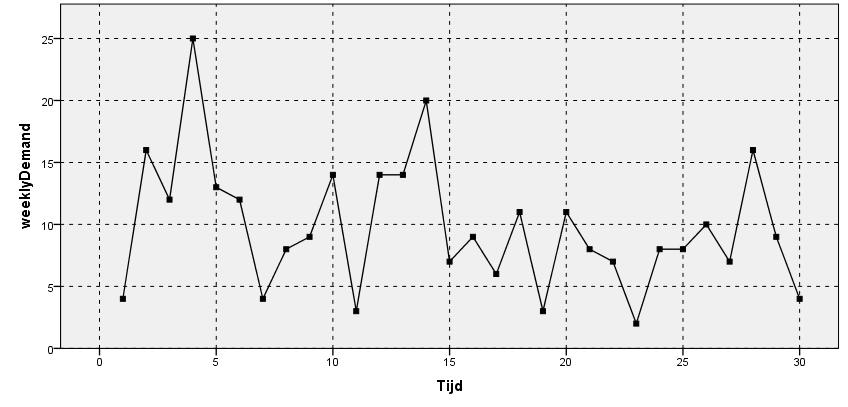
\includegraphics[width=.7\textwidth]{tijdreeks11}
  \end{figure}
\end{frame}

\begin{frame}
  \frametitle{Example: parameter estimation}
  
  \begin{itemize}
    \item We select the constant model of Equation~\ref{eq:time-series-constant}
    \item As an estimate for $b$ we select the mean of the first 20 observations:
    
    \[ \widehat{b} = \frac{1}{20} \sum_{t = 1}^{20} x_{t}= 10.75 \]
    
  \end{itemize}
  
  \centering
  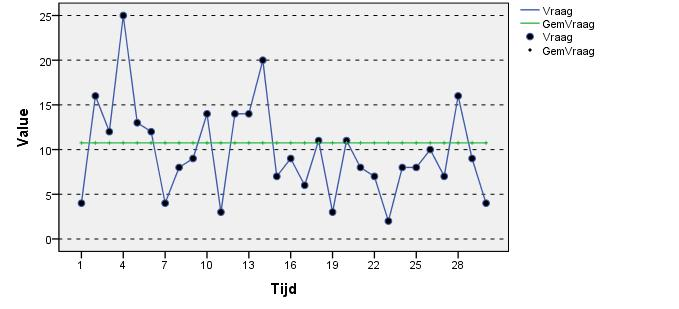
\includegraphics[width=.7\textwidth]{tijdreeks21.jpg}
\end{frame}

\begin{frame}
  \frametitle{Example: parameter estimation}
  
  You choose which observations you use to determine $\widehat{b}$, e.g.:
  
  \begin{itemize}
    \item $\widehat{b} = \frac{1}{10} \sum_{10}^{20} x_{t} = 10.18$
    \item $\widehat{b} = \frac{1}{5} \sum_{15}^{20} x_{t} = 7.83$
  \end{itemize}
  
\end{frame}

\section{Moving average}

\subsection{Simple moving average}

\begin{frame}
  \frametitle{Moving average}
  
  \alertbox{The moving average is a series of \textbf{averages (means)} of the last $m$ observations}
  
  \small
  
  \begin{itemize}
    \item Notation: SMA
    \item Hide short-term fluctuations and show long-term trends
    \item $m$ is the time range, and is the parameter of this method
  \end{itemize}
  
  \begin{equation}
  SMA(t) = \sum_{i=k}^{t} \frac{x_{i}}{m}
  \label{eq:movingAverage}
  \end{equation}
  
  with $k = t - m + 1$.
\end{frame}

\begin{frame}[plain]
  \frametitle{Example: ``Golden cross''}
  
  Moving averages are used in the \textbf{technical analysis} of stock prices to discover trends:
  
  \begin{center}
    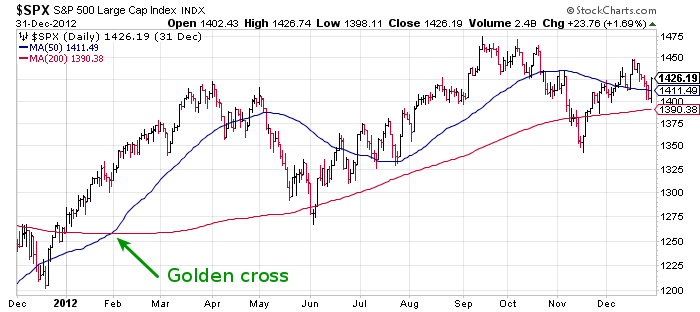
\includegraphics[height=.6\textheight]{tijdreeks-golden-cross}
  \end{center}
\end{frame}

\note{%
  \footnotesize
  Deze grafiek is de koers van de S\&P500 index (vergelijk met onze Bel-20) voor december 2011 tot eind 2012. In de grafiek worden de SMA's van de prijs bij sluitingstijd van de 50 en 200 laatste beursdagen gegeven (notatie: MA(50) en MA(200)). Wanneer de markt in een dalende trend zit (``\textbf{bear market}''), ligt de MA(200) boven MA(50) (zie linkse deel van de tekening).
  
  In februari 2012 ging MA(50) boven de MA(200), een verschijnsel dat ``\textbf{the golden cross}'' genoemd wordt. De stijging van de index was al enkele maanden eerder ingezet, maar de MA's reageren uiteraard trager.
  
  Een \textbf{golden cross} is een indicator dat de markt (of een specifiek aandeel) in een lange-termijn stijgende trend zit (``\textbf{bull market}''). In dit geval duurt deze trend nog voort tot vandaag (voorjaar 2015).
  
  De MA(200)-lijn wordt dan beschouwd als ``steunpunt'', d.w.z.~een ondergrens voor het koerscijfer. Aan deze prijs is het aandeel heel interessant, stijgt de vraag en wordt de koers terug omhoog getrokken.
  
}

\begin{frame}
  \begin{table}
    \begin{tabular}{|llllllllll|}
      \hline
      ~       & 11   & 12   & 13   & 14   & 15   & 16   & 17   & 18   & 19   \\
      $x_{t}$ & 3    & 14   & 14   & 20   & 7    & 9    & 6    & 11   & 3    \\
      $X_{t}$ & 11.7 & 11.6 & 11.4 & 11.6 & 11.1 & 10.5 & 10.2 & 10.4 & 10.7 \\
      $e$     & -8.7 & 2.4  & 2.6  & 8.4  & -4.1 & -1.5 & -4.2 & 0.6  & -7.7 \\ \hline
    \end{tabular}
    \caption{Prediction error for a moving average $m = 10$}
    \label{tab:error}
  \end{table}
  
  A method for measuring the prediction error is calculating the mean of the deviations ($MAD$).
  
  \begin{equation}
  MAD = \frac{1}{n} \sum_{1}^{n} \left| e_{i} \right|
  \label{eq:MAD}
  \end{equation}
  
  You can also calculate the variance of the errors:
  
  \begin{equation}
  s^{2}_{e} = \frac{1}{m} \sum_{1}^{n} (e_{i} - \overline{e})^{2}
  \label{eq:varError}
  \end{equation}
\end{frame}

\subsection{Weighted moving average}

\begin{frame}
  \frametitle{Weighted moving average}
  
  \begin{itemize}
    \item For $SMA$, the weights of the observations are equal
    \item For a weighted moving average ($WMA$), more recent observations gain relatively more weight
    \item A specific form of this is exponential smoothing or the \textbf{exponential moving average} ($EMA$):
    \begin{equation}
    EMA(t) = \alpha x_{t-1} + (1-\alpha) EMA(t-1)
    \label{eq:singleExpSmooting}
    \end{equation}
    
    with $\alpha$ the smoothing constant ($0 < \alpha < 1$), and $t \geq 3$
  \end{itemize}
\end{frame}

\begin{frame}
  \frametitle{Exponential smoothing}
  
  Equation~\ref{eq:singleExpSmooting} is only valid from $t=3$. Determining the value of $EMA(2)$ is an important parameter.
  
  There are several options:
  
  \begin{itemize}
    \item $EMA(2) = x_1$
    \item $EMA(2) = \frac{1}{m} \sum_{i=1}^{m} x_i$ (so the mean of the first $m$ observations)
    \item make $EMA(2)$ equal to a specific objective
    \item \ldots
  \end{itemize}
\end{frame}

\begin{frame}
  \frametitle{Why ``\textit{exponential}''?}
  
  \begin{align*}
  EMA(t) &= \alpha x_{t-1} + (1-\alpha) EMA(t-1)                                           \\
  &= \alpha x_{t-1} + (1-\alpha)\left[\alpha x_{t-2} + (1-\alpha)EMA(t - 2)\right]  \\
  &= \alpha x_{t-1} + \alpha (1-\alpha)x_{t-2} + (1-\alpha)^{2} EMA(t - 2)          \\
  &  \text{or in general:} \\
  &= \alpha \sum_{i=1}^{t-2}(1-\alpha)^{i-1}x_{t-i} + (1-\alpha)^{t-2} EMA(2), t \geq 2
  \end{align*}
  
  In other words: older observations have an exponentially \\smaller weight.
\end{frame}

\begin{frame}
  \frametitle{Exponential smoothing}
  
  \begin{table}
    \centering
    \begin{tabular}{l|llll}
      $\alpha$ & $(1-\alpha)$ & $(1-\alpha)^{2}$ & $(1-\alpha)^{3}$ & $(1-\alpha)^{4}$ \\ \hline
      0.9   & 0.1       & 0.01             & 0.001                      & 0.0001           \\
      0.5   & 0.5       & 0.25             & 0.125                      & 0.062            \\
      0.1   & 0.9       & 0.81             & 0.729                      & 0.6561           \\
    \end{tabular}
    \caption{Values for $\alpha$ and $(1-\alpha)^{n}$}
    \label{tab:alpha}
  \end{table}
  The speed at which the old observations are ``forgotten'' depends on the value of $\alpha$. For a value of $\alpha$ close to 1, old observations are quickly forgotten , whereas for  $\alpha$ close to 0, this goes less fast.
\end{frame}


\begin{frame}
  \frametitle{Example}
  \begin{figure}[htbp]
    \centering
    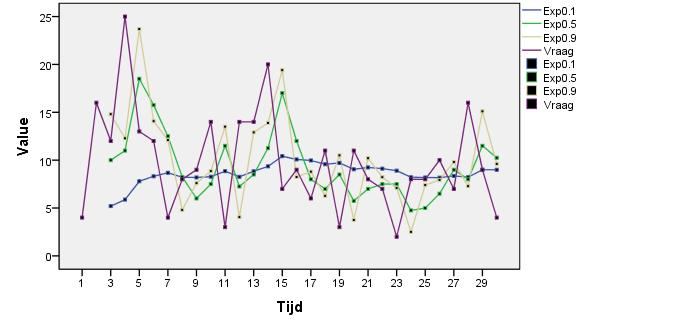
\includegraphics[width=\textwidth]{tijdreeks51}
    \caption{Basic exponential smoothing with $\alpha=0.1 , 0.5, 0.9$}
    \label{fig:tijdreeks51}
  \end{figure}
\end{frame}

\subsection{Double exponential smoothing}

\begin{frame}
  \frametitle{Double exponential smoothing}
  
  Basic exponential smoothing does not work well if there is a trend in the data
  
  \begin{figure}
    \centering
    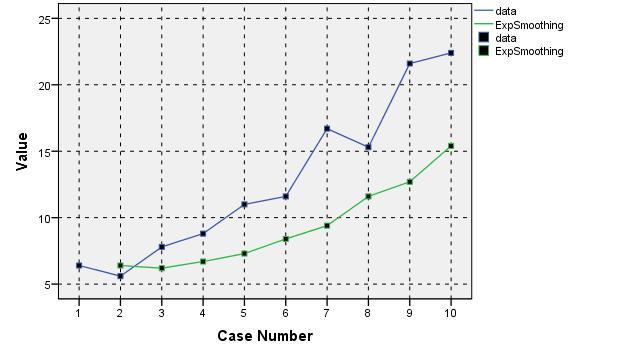
\includegraphics[width=.7\textwidth]{tijdreeks61}
    \caption{Exponential smoothing with a trend: the errors keep getting bigger}
    \label{fig:tijdreeks61}
  \end{figure}
  
\end{frame}


\begin{frame}
  \subsection{Double exponential smoothing}
  
  We add an additional term to model the trend. We use $s_t$ for the smoothing value, and $b_t$ for the estimation of the trend at time $t > 1$:
  
  \begin{align*}
  X_{t} & = \alpha x_{t} + (1-\alpha)(X_{t-1} + b_{t-1}) & 0 \leq \alpha \leq 1                            \\
  b_{t} & = \beta(X_{t}-X_{t-1}) + (1-\beta)b_{t-1}      & 0 \leq \beta \leq 1 
  \label{eq:doubleSmoothing}
  \end{align*}
  
  with $0 < \alpha < 1$ en $0 < \beta < 1$
  
  
  \begin{itemize}
    \item In the first equation, $b_{t-1}$ ensures that the trend is followed
    \item $X_{t}-X_{t-1}$ is positive or negative, this corresponds to an increasing/decreasing trend
  \end{itemize}
\end{frame}

\begin{frame}
  \subsection{Double exponential smoothing}
  Again, there are different options for selecting the initial values:
  
  \begin{align*}
  X_{1} &= x_{1} \\
  b_{1} &= x_{2} - x_{1} \\
  b_{1} &= \frac{1}{3}\left[ (x_{2} - x_{1}) + (x_{1} - x_{2}) + (x_{4} - x_{3}) \right]\\
  b_{1} &= \frac{x_{n} - x_{1}}{n-1}
  \end{align*}
  
\end{frame}

\subsubsection{Predicting}

\begin{frame}
  \frametitle{Predicting (forecasting)}
  
  To make a prediction (forecast) $F(t+1)$ for time $t+1$ we use:
  
  \[ F(t+1) = s_t + b_t \]
  
  or in general for time $t+m$:
  
  \[ F(t+m) = s_t + m b_t \]
\end{frame}

\begin{frame}
  \begin{figure}
    \centering
    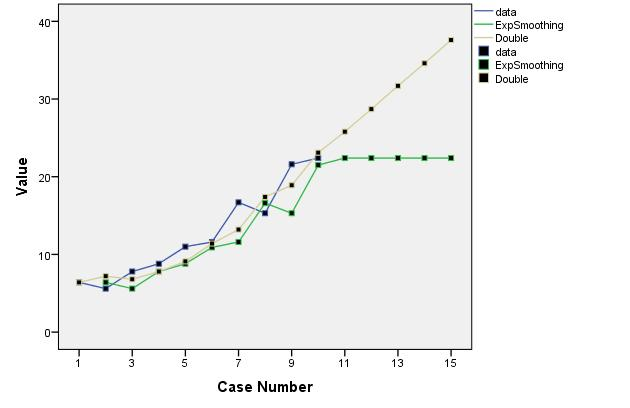
\includegraphics[width=\textwidth]{tijdreeks71}
    \caption{Basic and double exponential smoothing}
    \label{fig:tijdreeks71}
  \end{figure}
\end{frame}

\subsection{Triple exponential smoothing}

\begin{frame}
  \frametitle{Triple exponential smoothing}
  
  or the Holt-Winter method. This takes into account seasonality in the data. We note:
  
  \begin{itemize}
    \item $L$: length of the seasonal cycle (number of time units)
    \item $c_t$: term that models the seasonal variations
    \item $\gamma$: smoothing factor for the seasonal variation
  \end{itemize}
  
  \begin{align*}
  X_{t} &= \alpha \frac{x_{t}}{c_{t-L}} + (1-\alpha) (X_{t-1} + b_{t-1}) & \textnormal{Smoothing}\\
  b_{t} &= \beta (X_{t} - X_{t-1}) + (1-\beta)b_{t-1} & \textnormal{Trend smoothing} \\
  c_{t} &= \gamma \frac{x_{t}}{X_{t}} + (1-\gamma)c_{t-L} & \textnormal{Seasonal smoothing} \\
  \label{eq:HoltWinters}
  \end{align*}
  
\end{frame}

\begin{frame}
  \frametitle{Triple exponential smoothing}
  
  Prediction at time $t + m$:
  
  \[ F_{t+m} = (X_{t} + mb_{t})c_{t-L+m} \]
  
  For an implementation in Java, cfr. \url{https://github.com/bertvv/wintersmethod}
\end{frame}

\begin{frame}
  \frametitle{Example: predict sales figures}
  
  \centering
  \begin{tikzpicture}
  \begin{axis}[
  title=Observed Sales Figures,
  xlabel=Weekday,
  ylabel=SKUs,
  ]
  \addplot table [x index=0, y index=1, col sep=comma] {data/shoestore-sales.dat};
  \end{axis}
  \end{tikzpicture}
\end{frame}

\begin{frame}
  \frametitle{Example}
  
  Selected initial values:
  
  \begin{itemize}
    \item smoothing factors: $\alpha = 0.8, \beta = 0.8, \gamma = 0.3$
    \item $s_0 = 5849$, $b_0 = 123.3$
    \item $L = 7$ (weekly occurring), so we need 7 values to initialize $c_t$ (cfr. table)
  \end{itemize}
  
  \begin{table}
    \centering
    \begin{tabular}{l|l|l|l}
      mon ($c_0$) & tue ($c_1$) & wed ($c_2$) & thu ($c_3$)  \\
      1.245693 & 1.115265 & 1.088853 & 1.135378 \\
      \hline \hline
      fri ($c_4$)  & sat ($c_5$)  & sun ($c_6$)  & \\
      1.178552 & 1.229739 & 0.006520 &
    \end{tabular}
    \caption{Initial values for $c_t$}
    \label{tab:winters-init-c}
  \end{table}
\end{frame}

\begin{frame}
  \frametitle{Example: prediction}
  
  
  \begin{center}
    \begin{tikzpicture}
    \begin{axis}[
    scale=.8,
    title=Sales Figures,
    xlabel=Weekday,
    ylabel=SKUs,
    unbounded coords=jump,
    legend to name=bottomlegend,
    ]
    \addplot table [x index=0, y index=1, col sep=comma] {data/shoestore-sales.dat};
    \addlegendentry{Observed}
    \addplot table [x index=0, y index=2, col sep=comma] {data/shoestore-sales.dat};
    \addlegendentry{Estimated}
    \end{axis}
    \end{tikzpicture}
    
    \ref{bottomlegend}
  \end{center}
  
\end{frame}

\end{document}